\section{Clases de la API}

\begin{figure}[H]
    \centering
    \makebox[\textwidth][c]{
        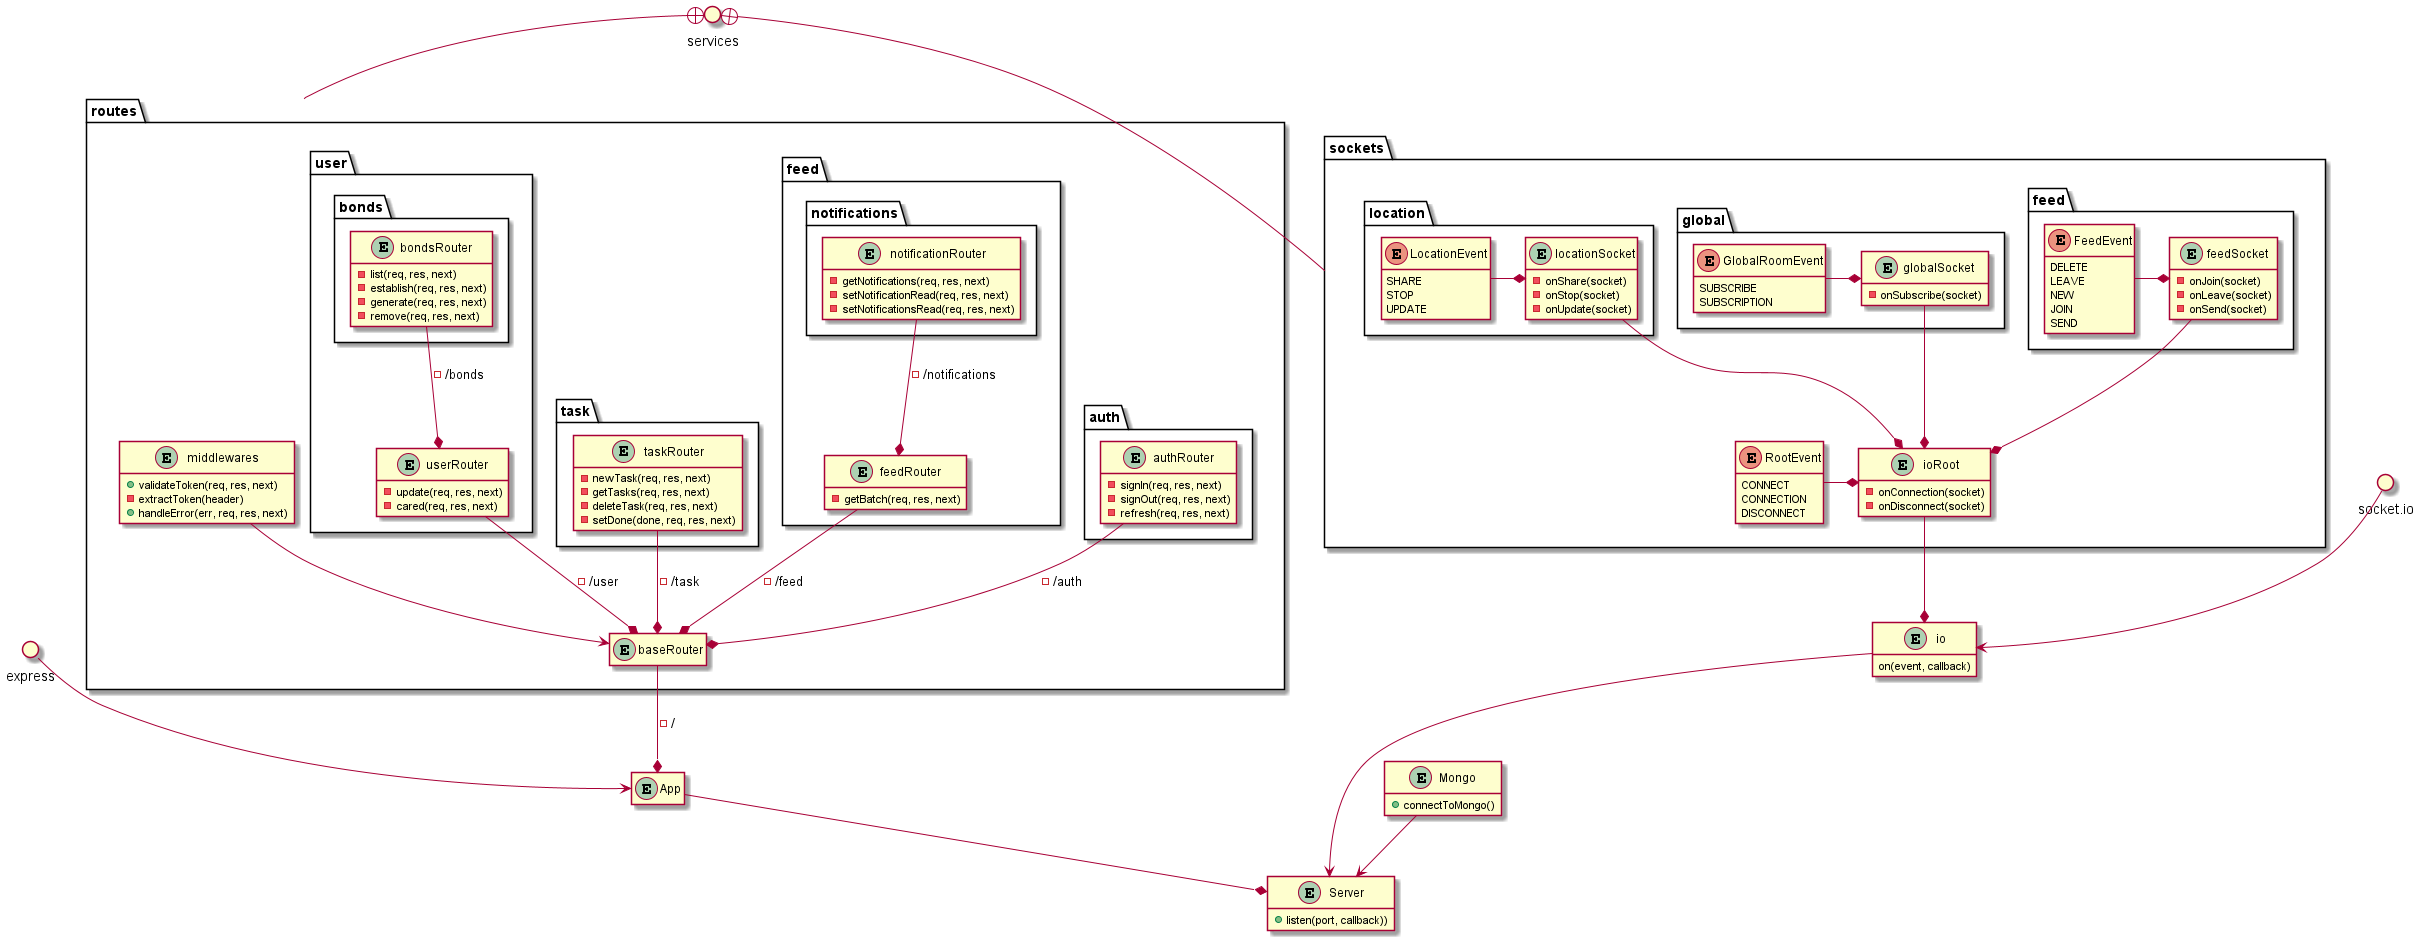
\includegraphics[width=1.2\textwidth]{images/Diseño/ClasesApiA.png}
    }
    \caption{Primera parte del diagrama de clases de la API}
    \label{fig:diagrama_clases_api_a}
\end{figure}

\begin{figure}[H]
    \centering
    \makebox[\textwidth][c]{
        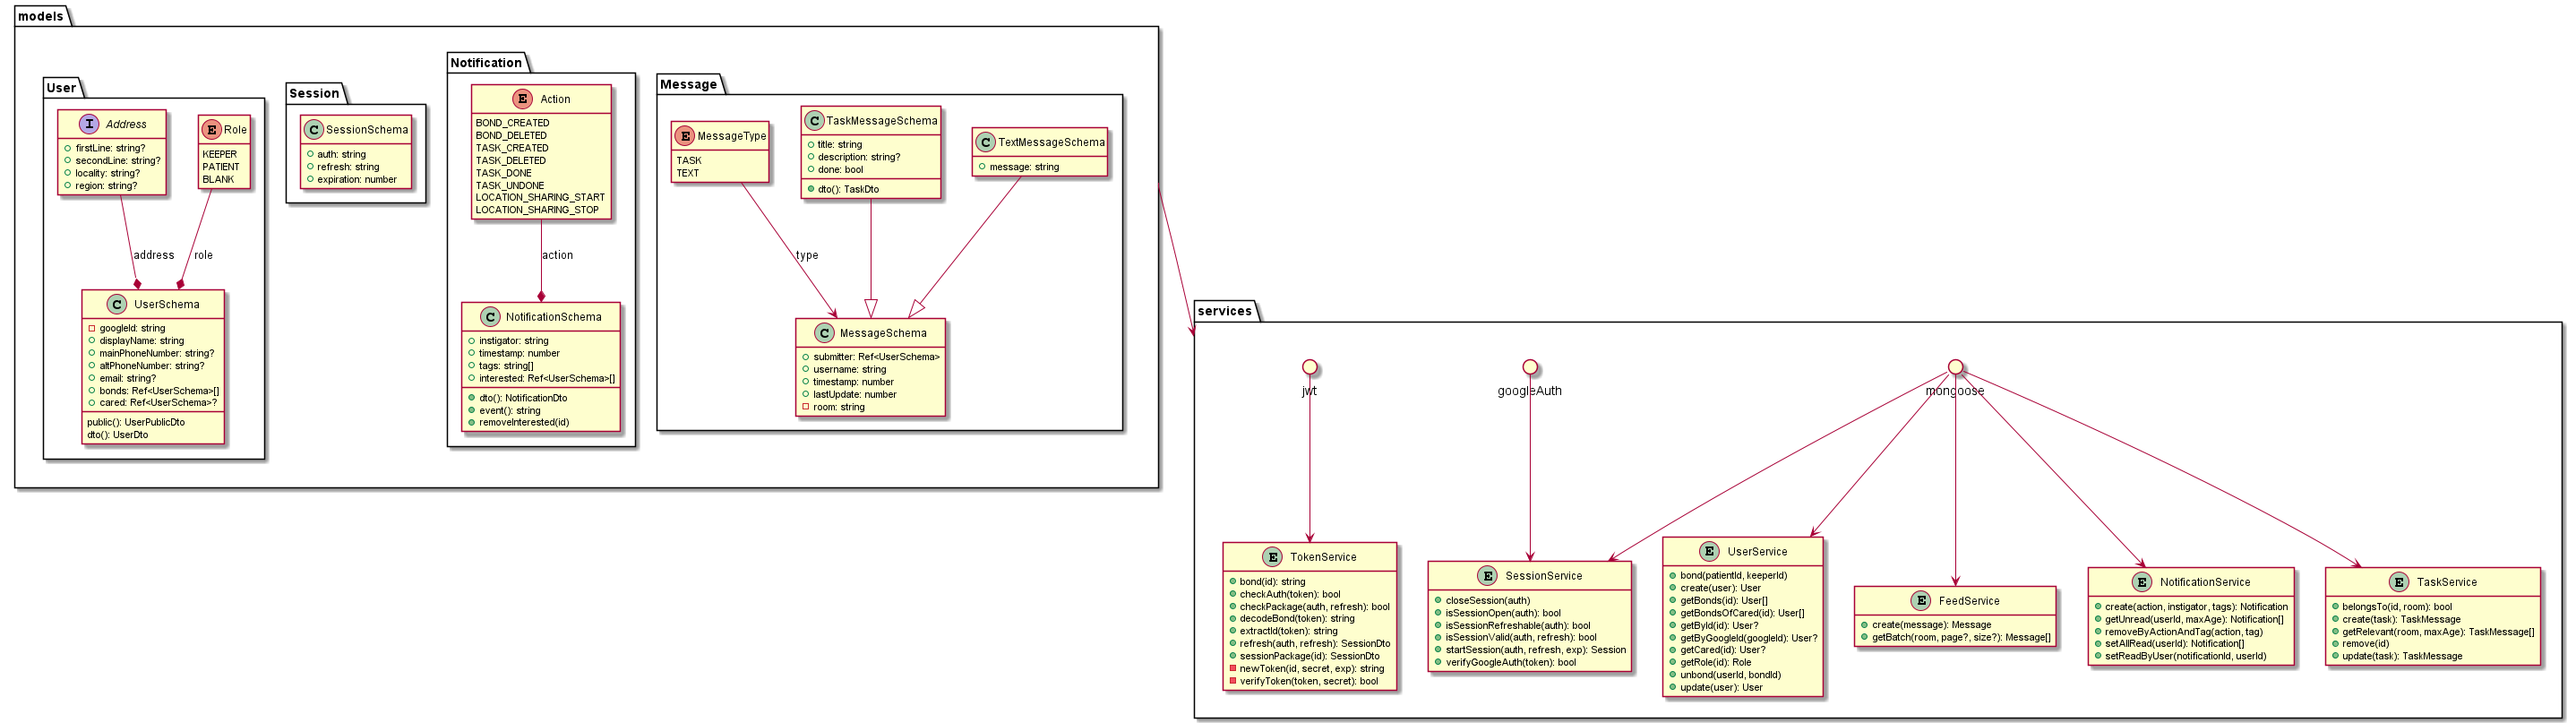
\includegraphics[width=1.2\textwidth]{images/Diseño/ClasesApiB.png}
    }
    \caption{Segunda parte del diagrama de clases de la API}
    \label{fig:diagrama_clases_api_b}
\end{figure}

\begin{figure}[H]
    \centering
    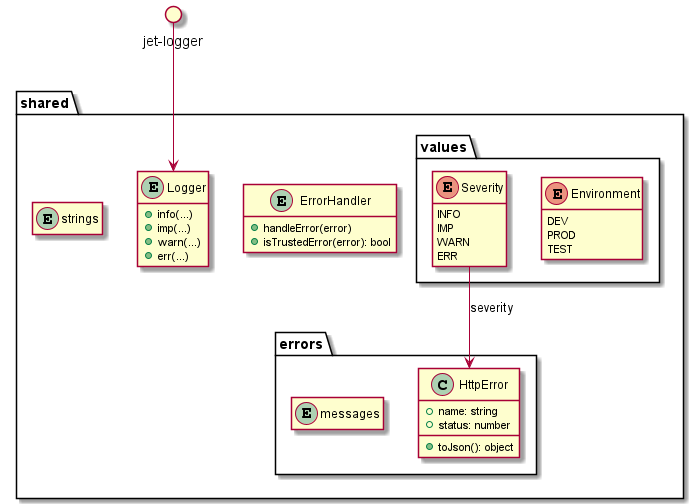
\includegraphics[width=0.3\textwidth]{images/Diseño/ClasesApiC.png}
    \caption{Tercera parte del diagrama de clases de la API}
    \label{fig:diagrama_clases_api_c}
\end{figure}

\subsection{Root}

\begin{longtable}{|p{0.25\textwidth} p{0.75\textwidth}|}
    \hline
    \multicolumn{2}{|l|}{\textbf{Server}} \\ \hline \hline
    Descripción      & Módulo principal del sistema. Inicializa todos los sistemas de la API en su lanzamiento desde el punto de entrada de la aplicación \\ \hline
    \multicolumn{2}{|l|}{Funciones} \\
    \emph{listen}  & Despliega el servidor en la direcciones y puerto especificados  \\ \hline
    \caption{Documentación de la entidad Server}
    \label{dis:api:server}
\end{longtable}

\begin{longtable}{|p{0.25\textwidth} p{0.75\textwidth}|}
    \hline
    \multicolumn{2}{|l|}{\textbf{App}} \\ \hline \hline
    Descripción      & Implementación del servidor Express, punto de entrada REST \\ \hline
    \caption{Documentación de la entidad App}
    \label{dis:api:app}
\end{longtable}

\begin{longtable}{|p{0.25\textwidth} p{0.75\textwidth}|}
    \hline
    \multicolumn{2}{|l|}{\textbf{Mongo}} \\ \hline \hline
    Descripción      & Módulo a cargo de la lógica relativa a la conexión de Mongoose con la base de datos \\ \hline
    \multicolumn{2}{|l|}{Funciones} \\
    \emph{connectToMongo}  & Crea la conexión con la base de datos remota  \\ \hline
    \caption{Documentación de la entidad Mongo}
    \label{dis:api:mongo}
\end{longtable}

\begin{longtable}{|p{0.25\textwidth} p{0.75\textwidth}|}
    \hline
    \multicolumn{2}{|l|}{\textbf{io}} \\ \hline \hline
    Descripción      & Implementación del servidor SocketIO, punto de entrada de los eventos WebSocket \\ \hline
    \multicolumn{2}{|l|}{Funciones} \\
    \emph{on}  & Define un evento y la función a realizar en el mismo  \\ \hline
    \caption{Documentación de la entidad io}
    \label{dis:api:io}
\end{longtable}

\subsection{Routes}

\begin{longtable}{|p{0.25\textwidth} p{0.75\textwidth}|}
    \hline
    \multicolumn{2}{|l|}{\textbf{baseRouter}} \\ \hline \hline
    Descripción      & Manejador raíz encargado de redireccionar las peticiones REST al manejador encargado de cada una según la ruta \\ \hline
    \caption{Documentación de la entidad baseRouter}
    \label{dis:api:base_router}
\end{longtable}

\begin{longtable}{|p{0.25\textwidth} p{0.75\textwidth}|}
    \hline
    \multicolumn{2}{|l|}{\textbf{authRouter}} \\ \hline \hline
    Descripción      & Manejador de las peticiones de /auth \\ \hline
    \multicolumn{2}{|l|}{Funciones} \\
    \emph{signIn}  & Crea una sesión para el usuario  \\ 
    \emph{signOut}  & Cierra la sesión de un usuario  \\ 
    \emph{refresh}  & Refresca la sesión del usuario  \\ \hline
    \caption{Documentación de la entidad authRouter}
    \label{dis:api:auth_router}
\end{longtable}

\begin{longtable}{|p{0.25\textwidth} p{0.75\textwidth}|}
    \hline
    \multicolumn{2}{|l|}{\textbf{feedRouter}} \\ \hline \hline
    Descripción      & Manejador de las peticiones de /feed \\ \hline
    \multicolumn{2}{|l|}{Funciones} \\
    \emph{getBatch}  & Devuelve el conjunto de mensajes solicitado por el usuario  \\ \hline
    \caption{Documentación de la entidad feedRouter}
    \label{dis:api:feed_router}
\end{longtable}

\begin{longtable}{|p{0.25\textwidth} p{0.75\textwidth}|}
    \hline
    \multicolumn{2}{|l|}{\textbf{notificationRouter}} \\ \hline \hline
    Descripción      & Manejador de las peticiones de /feed/notifications \\ \hline
    \multicolumn{2}{|l|}{Funciones} \\
    \emph{getNotifications}  & Devuelve las notificaciones pendientes del usuario  \\ 
    \emph{setNotificationRead}  & Marcar una notificación como leída  \\ 
    \emph{setNotificationsRead}  & Marca todas las notificaciones del usuario como leídas  \\ \hline
    \caption{Documentación de la entidad notificationRouter}
    \label{dis:api:notification_router}
\end{longtable}

\begin{longtable}{|p{0.25\textwidth} p{0.75\textwidth}|}
    \hline
    \multicolumn{2}{|l|}{\textbf{taskRouter}} \\ \hline \hline
    Descripción      & Manejador de las peticiones de /task \\ \hline
    \multicolumn{2}{|l|}{Funciones} \\
    \emph{newTask}  & Crea una nueva tarea  \\ 
    \emph{deleteTask}  & Elimina la tarea especificada  \\ 
    \emph{getTasks}  & Retorna las tareas relevantes relacionadas con el usuario  \\ 
    \emph{setTaskDone}  & Marca una tarea como hecha/no hecha  \\ \hline
    \caption{Documentación de la entidad taskRouter}
    \label{dis:api:task_router}
\end{longtable}

\begin{figure}[H]
\begin{longtable}{|p{0.25\textwidth} p{0.75\textwidth}|}
    \hline
    \multicolumn{2}{|l|}{\textbf{userRouter}} \\ \hline \hline
    Descripción      & Manejador de las peticiones de /user \\ \hline
    \multicolumn{2}{|l|}{Funciones} \\
    \emph{cared}  & Devuelve la información del paciente vinculado con el usuario  \\
    \emph{update}  & Actualiza la información del usuario  \\  \hline
    \caption{Documentación de la entidad userRouter}
    \label{dis:api:user_router}
\end{longtable}
\end{figure}

\begin{longtable}{|p{0.25\textwidth} p{0.75\textwidth}|}
    \hline
    \multicolumn{2}{|l|}{\textbf{bondsRouter}} \\ \hline \hline
    Descripción      & Manejador de las peticiones de /user/bonds \\ \hline
    \multicolumn{2}{|l|}{Funciones} \\
    \emph{list}  & Devuelve los vínculos del usuario  \\
    \emph{establish}  & Crea un vínculo entre usuarios  \\
    \emph{generate}  & Genera un código de vinculación  \\
    \emph{remove} & Elimina un vínculo entre usuarios \\ \hline
    \caption{Documentación de la entidad bondsRouter}
    \label{dis:api:bonds_router}
\end{longtable}

\subsection{Sockets}

\begin{longtable}{|p{0.25\textwidth} p{0.75\textwidth}|}
    \hline
    \multicolumn{2}{|l|}{\textbf{ioRoot}} \\ \hline \hline
    Descripción      & Manejador raíz encargado de los eventos de conexión y desconexión y de gestionar el registro de manejadores \\ \hline
    \caption{Documentación de la entidad ioRoot}
    \label{dis:api:io_root}
\end{longtable}

\begin{longtable}{|p{0.25\textwidth} p{0.75\textwidth}|}
    \hline
    \multicolumn{2}{|l|}{\textbf{RootEvent}} \\ \hline \hline
    Descripción      & Eventos de conexión al socket \\ \hline
    \multicolumn{2}{|l|}{Valores} \\
    \emph{CONNECT}  & Intento de conexión al socket  \\
    \emph{CONNECTION}  & Conexión exitosa al socket  \\
    \emph{DISCONNECT}  & Desconexión del socket \\ \hline
    \caption{Documentación del enumerado RootEvent}
    \label{dis:api:root_event}
\end{longtable}

\hspace{\textwidth}
\begin{longtable}{|p{0.25\textwidth} p{0.75\textwidth}|}
    \hline
    \multicolumn{2}{|l|}{\textbf{feedSocket}} \\ \hline \hline
    Descripción      & Manejador de la sala del Feed \\ \hline
    \multicolumn{2}{|l|}{Funciones} \\
    \emph{onJoin}  & Gestiona la entrada de un usuario en la sala  \\
    \emph{onLeave}  & Gestione el abandono de la sala de un usuario  \\
    \emph{onSend}  & Maneja el envío de un mensaje  \\ \hline
    \caption{Documentación de la entidad feedSocket}
    \label{dis:api:feed_socket}
\end{longtable}

\begin{longtable}{|p{0.25\textwidth} p{0.75\textwidth}|}
    \hline
    \multicolumn{2}{|l|}{\textbf{FeedEvent}} \\ \hline \hline
    Descripción      & Eventos de la sala del feed \\ \hline
    \multicolumn{2}{|l|}{Valores} \\
    \emph{DELETE}  & Eliminación de un mensaje  \\
    \emph{LEAVE}  & Abandono de la sala  \\
    \emph{NEW}  & Nuevo usuario en la sala  \\
    \emph{JOIN}  & Unión a la sala  \\
    \emph{SEND}  & Envío de un nuevo mensaje  \\ \hline
    \caption{Documentación del enumerado FeedEvent de la API}
    \label{dis:api:feed_event}
\end{longtable}

\begin{longtable}{|p{0.25\textwidth} p{0.75\textwidth}|}
    \hline
    \multicolumn{2}{|l|}{\textbf{globalSocket}} \\ \hline \hline
    Descripción      & Manejador de la sala Global \\ \hline
    \multicolumn{2}{|l|}{Funciones} \\
    \emph{onSubscribe}  & Gestiona la suscripción de un usuario a la sala \\ \hline
    \caption{Documentación de la entidad globalSocket}
    \label{dis:api:global_socket}
\end{longtable}

\begin{longtable}{|p{0.25\textwidth} p{0.75\textwidth}|}
    \hline
    \multicolumn{2}{|l|}{\textbf{GlobalEvent}} \\ \hline \hline
    Descripción      & Eventos de la sala global \\ \hline
    \multicolumn{2}{|l|}{Valores} \\
    \emph{SUBSCRIBE}  & Unión a la sala  \\
    \emph{SUBSCRIPTION} & Nuevo usuario en la sala  \\ \hline
    \caption{Documentación del enumerado GlobalEvent de la API}
    \label{dis:api:global_event}
\end{longtable}

\hspace{\textwidth}
\begin{longtable}{|p{0.25\textwidth} p{0.75\textwidth}|}
    \hline
    \multicolumn{2}{|l|}{\textbf{locationSocket}} \\ \hline \hline
    Descripción      & Manejador de la sala de la geolocalización \\ \hline
    \multicolumn{2}{|l|}{Funciones} \\
    \emph{onShare}  & Gestiona la entrada de un usuario en la sala  \\
    \emph{onStop}  & Gestione el abandono de la sala de un usuario  \\
    \emph{onUpdate}  & Maneja el envío de una localización  \\ \hline
    \caption{Documentación de la entidad locationSocket}
    \label{dis:api:location_socket}
\end{longtable}

\vspace{-15pt}
\begin{longtable}{|p{0.25\textwidth} p{0.75\textwidth}|}
    \hline
    \multicolumn{2}{|l|}{\textbf{LocationEvent}} \\ \hline \hline
    Descripción      & Eventos de la sala Location \\ \hline
    \multicolumn{2}{|l|}{Valores} \\
    \emph{SHARE}  & Unión a la sala  \\
    \emph{STOP} & Abandono de la sala  \\
    \emph{UPDATE} & Envío de una nueva ubicación  \\ \hline
    \caption{Documentación del enumerado LocationEvent de la API}
    \label{dis:api:location_event}
\end{longtable}

\vspace{-25pt}
\subsection{Services}

\begin{longtable}{|p{0.25\textwidth} p{0.75\textwidth}|}
    \hline
    \multicolumn{2}{|l|}{\textbf{FeedService}} \\ \hline \hline
    Descripción      & Servicio a cargo de los mensajes del feed \\ \hline
    \multicolumn{2}{|l|}{Funciones} \\
    \emph{create}  & Crea y persiste un nuevo mensaje  \\
    \emph{getBatch}  & Devuelve la lista de mensajes especificada  \\ \hline
    \caption{Documentación de la clase FeedService de la API}
    \label{dis:api:feed_service}
\end{longtable}

\vspace{-15pt}
\begin{longtable}{|p{0.3\textwidth} p{0.7\textwidth}|}
    \hline
    \multicolumn{2}{|l|}{\textbf{NotificationService}} \\ \hline \hline
    Descripción      & Servicio a cargo de las notificaciones \\ \hline
    \multicolumn{2}{|l|}{Funciones} \\
    \emph{create}  & Crea y persiste una nueva notificación  \\
    \emph{getUnread}  & Devuelve la lista de notificaciones no leídas de un usuario  \\
    \emph{removeByActionAndTag}  & Elimina las notificaciones que tienen la misma acción y etiquetas  \\
    \emph{setAllRead}  & Marca todas las notificaciones de un usuario como leídas  \\
    \emph{setReadByUser}  & Marca una notificación como leída  \\ \hline
    \caption{Documentación de la clase NotificationService}
    \label{dis:api:notification_service}
\end{longtable}

\begin{longtable}{|p{0.25\textwidth} p{0.75\textwidth}|}
    \hline
    \multicolumn{2}{|l|}{\textbf{SessionService}} \\ \hline \hline
    Descripción      & Servicio a cargo de las sesiones de usuario \\ \hline
    \multicolumn{2}{|l|}{Funciones} \\
    \emph{closeSession}  & Cierra la sesión especificada  \\
    \emph{isSessionOpen}  & Comprueba si una sesión está activa  \\
    \emph{isSessionRefreshable}  & Comprueba si una sesión se puede refrescar  \\
    \emph{isSessionValid}  & Comprueba si una sesión es válida  \\
    \emph{startSession}  & Crea una nueva sesión de usuario  \\
    \emph{verifyGoogleAuth}  & Verifica un token de autenticación de Google  \\ \hline
    \caption{Documentación de la clase SessionService}
    \label{dis:api:session_service}
\end{longtable}

\vspace{-10pt}
\begin{longtable}{|p{0.25\textwidth} p{0.75\textwidth}|}
    \hline
    \multicolumn{2}{|l|}{\textbf{TaskService}} \\ \hline \hline
    Descripción      & Servicio a cargo de las tareas \\ \hline
    \multicolumn{2}{|l|}{Funciones} \\
    \emph{belongsTo}  & Comprueba si la tarea pertenece a un usuario  \\
    \emph{create}  & Crea y persiste una nueva tarea  \\
    \emph{getRelevant}  & Devuelve la lista de tareas relevantes de un usuario  \\
    \emph{remove}  & Elimina la tarea especificada  \\
    \emph{update}  & Actualiza una tarea  \\ \hline
    \caption{Documentación de la clase TaskService de la API}
    \label{dis:api:task_service}
\end{longtable}

\vspace{-10pt}
\begin{longtable}{|p{0.25\textwidth} p{0.75\textwidth}|}
    \hline
    \multicolumn{2}{|l|}{\textbf{TokenService}} \\ \hline \hline
    Descripción      & Servicio para proveer y gestionar tokens \\ \hline
    \multicolumn{2}{|l|}{Funciones} \\
    \emph{bond}  & Genera un token de vinculación  \\
    \emph{checkAuth}  & Comprueba la validez de un token de autenticación  \\
    \emph{checkPackage}  & Comprueba la validez de una dupla de tokens de sesión  \\
    \emph{decodeBond}  & Descodifica un token de vinculación  \\
    \emph{extractId}  & Devuelve la ID de usuario almacenada en un token  \\
    \emph{newToken}  & Produce un nuevo token según la ID de usuario, el secreto y el tiempo de expiración  \\
    \emph{refresh}  & Genera una nueva tupla de tokens de sesión a partir una válida \\
    \emph{session}  & Genera una tupla de tokens de sesión nueva  \\
    \emph{verifyToken}  & Verifica la validez de un token  \\ \hline
    \caption{Documentación de la clase TokenService}
    \label{dis:api:token_service}
\end{longtable}

\begin{longtable}{|p{0.25\textwidth} p{0.75\textwidth}|}
    \hline
    \multicolumn{2}{|l|}{\textbf{UserService}} \\ \hline \hline
    Descripción      & Servicio a cargo de los datos de usuario \\ \hline
    \multicolumn{2}{|l|}{Funciones} \\
    \emph{bond}  & Crea un vínculo entre usuarios  \\
    \emph{create}  & Crea un nuevo usuario \\
    \emph{getBonds}  & Devuelve los vínculos de un usuario  \\
    \emph{getBondsOfCared}  & Devuelve los vínculos del paciente vinculado  \\
    \emph{getById}  & Retorna el usuario con la identidad especificada  \\
    \emph{getByGoogleId}  & Retorna el usuario con la identidad de Google especificada  \\
    \emph{getCared}  & Devuelve el paciente vinculado de un usuario  \\
    \emph{getRole}  & Devuelve el rol de un usuario  \\
    \emph{unbond} & Elimina el vínculo entre dos usuarios \\
    \emph{update}  & Actualiza los datos de un usuario  \\ \hline
    \caption{Documentación de la clase UserService de la API}
    \label{dis:api:user_service}
\end{longtable}

\vspace{-30pt}
\subsection{Models}

\vspace{-10pt}
\begin{longtable}{|p{0.5\textwidth} p{0.5\textwidth}|}
    \hline
    \multicolumn{2}{|l|}{\textbf{Action}} \\ \hline \hline
    Descripción      & Accciones notificables \\ \hline
    \multicolumn{2}{|l|}{Valores} \\
    \emph{BOND\textunderscore CREATED}  & Creación de un vínculo  \\
    \emph{BOND\textunderscore DELETED}  & Eliminación de un vínculo  \\
    \emph{TASK\textunderscore CREATED}  & Creación de una tarea  \\
    \emph{TASK\textunderscore DELETED}  & Eliminación de una tarea  \\
    \emph{TASK\textunderscore DONE}  & Actualización de una tarea a hecha  \\
    \emph{TASK\textunderscore UNDONE}  & Actualización de una tarea a no hecha  \\
    \emph{LOCATION\textunderscore SHARING\textunderscore START}  & Ubicación empezando a ser compartida  \\
    \emph{LOCATION\textunderscore SHARING\textunderscore STOP}  & Ubicación dejando de ser compartida  \\ \hline
    \caption{Documentación del enumerado Action de la API}
    \label{dis:api:action}
\end{longtable}

\vspace{-20pt}
\begin{longtable}{|p{0.25\textwidth} p{0.75\textwidth}|}
    \hline
    \multicolumn{2}{|l|}{\textbf{Address}} \\ \hline \hline
    Descripción      & Abstracción de direcciones postales \\ \hline
    \multicolumn{2}{|l|}{Propiedades} \\
    \emph{firstLine}  & Primera línea (por ejemplo, calle y número)  \\
    \emph{secondLine}  & Segunda línea (por ejemplo, piso y puerta)  \\
    \emph{locality}  & Localidad  \\
    \emph{region}  & Región (por ejemplo, provincia o estado)  \\ \hline
    \caption{Documentación de la interfaz Address de la API}
    \label{dis:api:address}
\end{longtable}

\begin{longtable}{|p{0.25\textwidth} p{0.75\textwidth}|}
    \hline
    \multicolumn{2}{|l|}{\textbf{MessageType}} \\ \hline \hline
    Descripción      & Tipos de mensajes \\ \hline
    \multicolumn{2}{|l|}{Valores} \\
    \emph{TASK}  & Tarea  \\
    \emph{TEXT}  & Mensaje de texto  \\ \hline
    \caption{Documentación del enumerado MessageType de la API}
    \label{dis:api:message_type}
\end{longtable}

\begin{longtable}{|p{0.25\textwidth} p{0.75\textwidth}|}
    \hline
    \multicolumn{2}{|l|}{\textbf{MessageSchema}} \\ \hline \hline
    Descripción      & Esquema base de los mensajes \\ \hline
    \multicolumn{2}{|l|}{Propiedades} \\
    \emph{submitter}  & Referencia a la entidad del autor  \\
    \emph{username}  & Nombre del autor \\
    \emph{timestamp}  & Instante de envío \\
    \emph{lastUpdate}  & Última actualización  \\
    \emph{room}  & Sala de envío  \\ \hline
    \caption{Documentación del esquema de Message de la API}
    \label{dis:api:message}
\end{longtable}

\begin{longtable}{|p{0.25\textwidth} p{0.75\textwidth}|}
    \hline
    \multicolumn{2}{|l|}{\textbf{NotificationSchema}} \\ \hline \hline
    Descripción      & Esquema de las notificaciones de la aplicación \\ \hline
    \multicolumn{2}{|l|}{Propiedades} \\
    \emph{action}  & Acción a notificar  \\
    \emph{instigator}  & Autor de la acción  \\
    \emph{timestamp}  & Instante de realización de la acción  \\
    \emph{tags}  & Etiquetas con información extra de la notificación  \\
    \emph{interested}  & Lista de usuarios receptores de la notificación  \\ \hline
    \multicolumn{2}{|l|}{Funciones} \\
    \emph{dto}  & Devuelve un NotificationDto de la notificación  \\
    \emph{event}  & Devuelve el código de evento del WebSocket \\
    \emph{removeInterested}  & Elimina al usuario especificado de la lista de interesados  \\ \hline
    \caption{Documentación del esquema de Notification de la API}
    \label{dis:api:notification}
\end{longtable}

\newpage
\begin{longtable}{|p{0.25\textwidth} p{0.75\textwidth}|}
    \hline
    \multicolumn{2}{|l|}{\textbf{Role}} \\ \hline \hline
    Descripción      & Roles de los usuarios \\ \hline
    \multicolumn{2}{|l|}{Valores} \\
    \emph{PATIENT}  & Pacientes  \\
    \emph{KEEPER}  & Cuidadores  \\
    \emph{BLANK}  & Sin rol  \\ \hline
    \caption{Documentación del enumerado Role de la API}
    \label{dis:api:role}
\end{longtable}

\begin{longtable}{|p{0.25\textwidth} p{0.75\textwidth}|}
    \hline
    \multicolumn{2}{|l|}{\textbf{SessionSchema}} \\ \hline \hline
    Descripción      & Esquema de una sesión de usuario \\ \hline
    \multicolumn{2}{|l|}{Propiedades} \\
    \emph{auth}  & Token de autenticación de la sesión  \\
    \emph{refresh}  & Token de refresco de la sesión  \\
    \emph{expiration}  & Instante de expiración de la sesión  \\ \hline
    \caption{Documentación del esquema de Session de la API}
    \label{dis:api:session}
\end{longtable}

\begin{longtable}{|p{0.25\textwidth} p{0.75\textwidth}|}
    \hline
    \multicolumn{2}{|l|}{\textbf{TaskMessageSchema}} \\ \hline \hline
    Descripción      & Esquema de una tarea \\ \hline
    \multicolumn{2}{|l|}{Propiedades} \\
    \emph{title}  & Título  \\
    \emph{description}  & Descripción  \\
    \emph{done}  & Estado: hecha/no hecha  \\ \hline
    \multicolumn{2}{|l|}{Funciones} \\
    \emph{dto}  & Devuelve un TaskDto de la tarea  \\ \hline
    \caption{Documentación del esquema de TaskMessage de la API}
    \label{dis:api:task_message}
\end{longtable}

\begin{longtable}{|p{0.25\textwidth} p{0.75\textwidth}|}
    \hline
    \multicolumn{2}{|l|}{\textbf{TextMessageSchema}} \\ \hline \hline
    Descripción      & Esquema de los mensajes de texto del Feed \\ \hline
    \multicolumn{2}{|l|}{Propiedades} \\
    \emph{message}  & Mensaje enviado  \\ \hline
    \caption{Documentación del esquema de TextMessage de la API}
    \label{dis:api:text_message}
\end{longtable}

\begin{longtable}{|p{0.25\textwidth} p{0.75\textwidth}|}
    \hline
    \multicolumn{2}{|l|}{\textbf{UserSchema}} \\ \hline \hline
    Descripción      & Esquema de los usuarios de la aplicación \\ \hline
    \multicolumn{2}{|l|}{Propiedades} \\
    \emph{role}  & Rol  \\
    \emph{googleId}  & Identidad de Google  \\
    \emph{displayName}  & Nombre para mostrar al resto de usuarios  \\
    \emph{mainPhoneNumber}  & Teléfono principal  \\
    \emph{altPhoneNumber}  & Teléfono alternativo  \\
    \emph{address}  & Dirección postal  \\
    \emph{email}  & Dirección electrónica  \\
    \emph{bonds}  & Lista de usuarios vinculados de los pacientes  \\
    \emph{cared}  & Usuario vinculado de los cuidadores  \\ \hline
    \caption{Documentación del esquema de User de la API}
    \label{dis:api:user}
\end{longtable}

\subsection{Shared}

\begin{longtable}{|p{0.25\textwidth} p{0.75\textwidth}|}
    \hline
    \multicolumn{2}{|l|}{\textbf{Logger}} \\ \hline \hline
    Descripción      & Encapsulación de la lógica del registro  \\ \hline
    \multicolumn{2}{|l|}{Funciones} \\
    \emph{info}  & Registra un mensaje de información  \\
    \emph{imp}  & Registra un mensaje importante  \\
    \emph{warn}  & Registra un mensaje de advertencia  \\
    \emph{err}  & Registra un mensaje de error  \\  \hline
    \caption{Documentación de la entidad Logger}
    \label{dis:api:logger}
\end{longtable}

\begin{longtable}{|p{0.25\textwidth} p{0.75\textwidth}|}
    \hline
    \multicolumn{2}{|l|}{\textbf{ErrorHandler}} \\ \hline \hline
    Descripción      & Manejador de errores  \\ \hline
    \multicolumn{2}{|l|}{Funciones} \\
    \emph{handleError}  & Gestiona y procesa un error  \\
    \emph{isTrustedError}  & Comprueba si es un error conocido  \\  \hline
    \caption{Documentación de la entidad ErrorHandler}
    \label{dis:api:error_handler}
\end{longtable}

\newpage
\begin{longtable}{|p{0.25\textwidth} p{0.75\textwidth}|}
    \hline
    \multicolumn{2}{|l|}{\textbf{HttpError}} \\ \hline \hline
    Descripción      & Errores con respuesta HTTP definida  \\ \hline
    \multicolumn{2}{|l|}{Propiedades} \\
    \emph{name}  & Nombre  \\
    \emph{severity}  & Severidad  \\
    \emph{status}  & Código de estado HTTP  \\ \hline
    \multicolumn{2}{|l|}{Funciones} \\
    \emph{toJson}  & Devuelve un JSON para enviar el error como respuesta  \\  \hline
    \caption{Documentación de la clase HttpError}
    \label{dis:api:http_error}
\end{longtable}

\begin{longtable}{|p{0.25\textwidth} p{0.75\textwidth}|}
    \hline
    \multicolumn{2}{|l|}{\textbf{Severity}} \\ \hline \hline
    Descripción      & Severidad \\ \hline
    \multicolumn{2}{|l|}{Valores} \\
    \emph{INFO}  & Información  \\
    \emph{IMP}  & Información importante  \\
    \emph{WARN}  & Advertencia  \\
    \emph{ERROR}  & Error severo  \\ \hline
    \caption{Documentación del enumerado Severity de la API}
    \label{dis:api:severity}
\end{longtable}

\begin{longtable}{|p{0.25\textwidth} p{0.75\textwidth}|}
    \hline
    \multicolumn{2}{|l|}{\textbf{Environment}} \\ \hline \hline
    Descripción      & Entornos de ejecución \\ \hline
    \multicolumn{2}{|l|}{Valores} \\
    \emph{DEV}  & Desarrollo  \\
    \emph{PROD}  & Producción  \\
    \emph{TEST}  & Pruebas  \\ \hline
    \caption{Documentación del enumerado Environment de la API}
    \label{dis:api:environment}
\end{longtable}